\chapter{Strukturierte Programmierung} \label{chp:funcs}
\epigraph{Before software can be reusable it first has to be usable.}{Ralph Johnson}

Viele Aufgaben wiederholen sich oder lassen sich verallgemeinern. Folgender Code berechnet beispielsweise den Wert von Eulers Zahl, also $\exp(1)$, kann aber auch dazu verwendet werden, andere Potenzen von e zu finden:

\begin{codebox}[Beispiel: Berechnung von Eulers Zahl]
\begin{minted}[linenos]{c}
#include <stdio.h>
#include <math.h>

int main () {
  double x0 = 1.0;
  
  int    accuracy = 20;
  double x        = 1.0;
  double d        = 1.0;
  double e        = 1.0;
  
  for (int i=1; i<accuracy; i++) {
    x *= x0;
    d *= i;
    e += x / d;
  }
  
  printf("Manuell: %10.8lf\n", e);
  printf("Mathlib: %10.8lf\n", exp(x0));
}
\end{minted}
\end{codebox}

\begin{cmdbox}[Ausführungseispiel: Berechnung von Eulers Zahl]
\begin{minted}{text}
Manuell: 2.71828183
Mathlib: 2.71828183
\end{minted}
\end{cmdbox}

Zeile 18 zeigt sowohl, dass dieser Code das gewünschte Ergebnis liefert, aber auch, dass es möglich sein sollte, solchen Code kompakt zu einem eigenen Befehl (hier \texttt{exp}) zusammenzufassen. In diesem Kapitel werden wir sehen, wie wir solche \emph{Funktionen} schreiben.

\section{Scopes} \label{sec:Scopes}
Die Funktionen, die wir selbst definieren werden, sollen vom restlichen Programmcode unabhängig sein. Das bedeutet, dass Variablen, die wir für in unserer Funktion benuzten keine anderen Werte überschreiben sollen, die wir im restlichen Programm benutzen. Dies soll für alle Programme gelten, die wir je schreiben, gleich, welche Variablennamen darin vorkommen. Um dies zu ermöglichen, existiert in C das Konzept von \emph{Scopes}:

Scopes sind Code-Abschnitte, innerhalb derer Variablen existieren, \ie innerhalb derer die Variablen über ihren Namen benutzt werden können. Variablen, die innerhalb eines Scopes deklariert wurden, \enquote{existieren} außerhalb dieses Scopes nicht. Scopes werden durch \{geschweifte Klammern\} eingegrenzt.

\begin{codebox}[Beispiel: Scopes (1)]
\begin{minted}[linenos]{c}
#include <stdio.h>

int main () {
  int x = 1;
  
  {
    int y = 2;
    printf("%d\n", y);
  }
  
  // printf("%d\n", y); -- Fehler: y nicht deklariert
}
\end{minted}
\end{codebox}

Die Variable \texttt{y} existiert nur Zwischen Zeile 7 (wo sie deklariert wird) und Zeile 9 (wo der Scope endet, innerhalb derer \texttt{y} \enquote{lebt}). Daher würde Zeile 11 einen Compiler-Fehler erzeugen, da auf eine nicht deklarierte Variable verwiesen wird.

Variablen sind \enquote{nach innen sichtbar}. Das bedeutet, dass die Variable \texttt{x} auch innerhalb des Scopes gelesen oder verändert werden kann, da sie außerhalb des Scopes deklariert wurde und nach innen \enquote{fortlebt}:

\begin{codebox}[Beispiel: Scopes (2)]
\begin{minted}[linenos]{c}
#include <stdio.h>

int main () {
  int x = 1;
  
  {
    int y = 2;
    printf("%d\n", x);  // kein Problem -- Sichtbarkeit nach innen.
    printf("%d\n", y);
  }
  
  // printf("%d\n", y); -- Fehler: y nicht deklariert
}
\end{minted}
\end{codebox}

Innerhalb von Scopes dürfen Namen auch neu vergeben werden. Das heißt, dass innerhalb des Scopes eine eigene Variable \texttt{x} deklariert werden darf. Die alte Variable \texttt{x} existiert weiterhin, ist aber unter diesem Namen nicht mehr ansprechbar. Stattdessen ist das neue \texttt{x} innerhalb des Scopes komplett unabhängig von dem \texttt{x} außerhalb, und existiert ebenso wie \texttt{y} nur innerhalb des Scopes:

\begin{codebox}[Beispiel: Scopes (3)]
\begin{minted}[linenos]{c}
#include <stdio.h>

int main () {
  int x = 1;
  
  {
    int y = 2;
    printf("%d\n", x);   // Sichtbarkeit nach innen -- 1 wird angezeigt
    printf("%d\n", y);
    
    double x = 5.0;
    printf("%lf\n", x);  // neue Variable wird unter dem Namen x angesprochen
  }
  
  printf("%d\n", x);     // alte Variable wird angesprochen -- Ausgabe 1
}
\end{minted}
\end{codebox}

\begin{cmdbox}[Ausführungseispiel: Scopes (3)]
\begin{minted}{text}
1
2
5.000000
1
\end{minted}
\end{cmdbox}

Scopes können (nahezu) beliebig tief ineinander verschachtelt werden und können auch \enquote{nebeineinander} stehen. Scopes, die auf gleicher Ebene nebeneinander stehen \enquote{sehen ihren Inhalt nicht}, \ie die Variablen, die in einem Scope deklariert werden können nicht von einem anderen Scope gelesen werden:

\begin{codebox}[Beispiel: Scopes (4)]
\begin{minted}[linenos]{c}
#include <stdio.h>

int main () {
  int x = 1;
  
  {
    int y = 2;
    printf("%d\n", x);     // Sichtbarkeit nach innen -- 1 wird angezeigt
    printf("%d\n", y);
    
    double x = 5.0;
    printf("%lf\n", x);    // neue Variable
  }
\end{minted}
\end{codebox}
  
\begin{codebox}[]
\begin{minted}[linenos, firstnumber=last]{c}
  {
    // printf("%d\n", y);  // Fehler -- keine Sichtbarkeit in andere Scopes 
                           // gleicher Ebene
    printf("%d\n", x);     // Sichtbarkeit nach innen -- 1 wird angezeigt. 
                           // Die double-Variable x ist "vergessen"
                           
    double x = 10.0;
    printf("%lf\n", x);    // neue Variable, wie zuvor.
  }
  printf("%d\n", x); 
}
\end{minted}
\end{codebox}

\section{Funktionen} \label{sec:funcs}
Eine \emph{Funktion} ist ein Programmabschnitt, der gewissermaßen unabhängig vom Rest des Codes existiert, und von jeder Stelle \emph{aufgerufen} werden kann. Wir haben mit \texttt{printf} und \texttt{scanf} schon zwei Funktionen im Detail kennengelernt; die Befehle der math-library sind ebenfalls solche Funktionen. Tatsächlich haben wir auch schon eine Funktion selbst geschrieben: die \mintinline{c}{int main ()} ist der Form nach ebenso ein solches Objekt.

Als Konzept ist eine Funktion eine Arbeitsanweisung, die einen Wert berechnet. Daher braucht eine Funktion zunächst einen \emph{Rückgabetyp}, also den Datentyp des Werts, der berechnet wird. Im Falle der \texttt{main} ist das eben \mintinline{c}{int}. Es folgt ein Name, über den die Funktion aufgerufen werden kann (wie eben \texttt{printf}) so wie eine \emph{Parameterliste}, \ie eine Liste von Variablen, abhängig von denen das Ergebnis der Funktion berechnet werden soll. Im Falle der \mintinline{c}{int main ()} ist dies eine leere Liste; wir werden bald Beispiele sehen, in denen Parameter mit übergeben werden.

Als erste Zeile einer Funktion folgen wir also der Syntax:
\begin{codebox}[Syntax: Deklaration von Funktionen]
Rückgabetyp Funktionsname(Parameterliste) \{...
\end{codebox}
Wir nennen dieses Set von Informationen (Rückgabetyp, Funktionsname und Parameterliste) auch den \emph{Prototyp} der Funktion. Verwandt damit ist der Begriff der \emph{Signatur}, die nur Rückgabetyp und Parameterliste beschreibt.

Die Parameterliste ist eine durch Kommata getrennte Liste von Datentypen und Bezeichnern (also Variablennamen). Diese Variablennamen sind unabhängig vom Rest des Codes: Eine Funktion öffnet einen eigenen Scope. In der Parameterliste werden die Variablen also erst deklariert. Wir können etwa folgenden Prototypen für Funktion vorschlagen, die die Exponentialfunktion berechnet:

\begin{codebox}[Signatur der Funktion \texttt{myExp}]
\begin{minted}{c}
double myExp(double x0, int accuracy) {...
\end{minted}
\end{codebox}

Nach der Funktionssignatur folgt -- eingeschlossen in \{geschweifte Klammern\} -- der \emph{Function-Body}. Dabei handelt es sich um beliebigen C-Code, wie wir ihn bisher schon kennen gelernt haben. Teil dieses Codes muss an irgend einer Stelle die Anweisung \mintinline{c}{return expression} sein. Diese Anweisung sorgt dafür, dass das \emph{aufrufende Programm} den berechneten Wert \texttt{expression} empfängt und die Funktion verlassen wird\footnote{Eine Funktion, die keine \mintinline{c}{return}-Anweisung enthält, wird ebenso verlassen, sobald ihre letzte Zeile ausgeführt wird. Allerdings kann dann keiner der berechneten Werte vom Hauptprogramm empfangen werden. Stattdessen erhält die aufrufende Stelle einen zufälligen Wert, wie bei einer uninitialisierten Variable.}. Folgendes Beispiel zeigt eine mögliche Umsetzung der Funktion \texttt{myExp}:

\begin{codebox}[Beispiel: Funktion \texttt{myExp}]
\begin{minted}[linenos]{c}
double myExp(double x0, int accuracy) {
  double x           = 1.0;
  double denominator = 1.0;
  double result      = 1.0;
  
  for (int i=1; i<accuracy; i++) {
    x           *= x0;
    denominator *= i;
    result      += x / denominator;
  }
  
  return result;
}
\end{minted}
\end{codebox}

Die Variablen \texttt{x0} und \texttt{accuracy} werden also schon im Funktions-Prototypen deklariert; \texttt{x}, \texttt{denominator} und \texttt{result} folgen im Funktions-Body. Alle diese fünf Variablen gehören demselben Scope an.

Um eine Funktion aufzurufen, setzen wir einfach ihren Namen, gefolgt von der Parameterliste in runden Klammern (). Beim Aufruf schreiben wir in die Parameterliste die Werte oder Ausdrücke, mit denen wir rechnen wollen. Diese Werte werden dann zuerst an die Speicherstellen des Funktion-Scopes kopiert, bevor der Code ausgeführt wird.

\begin{codebox}[Beispiel: Funktion \texttt{myExp} in Anwendung]
\begin{minted}[linenos]{c}
#include <stdio.h>
#include <math.h>

double myExp(double x0, int accuracy) {
  double x           = 1.0;
  double denominator = 1.0;
  double result      = 1.0;
  
  for (int i=1; i<accuracy; i++) {
    x           *= x0;
    denominator *= i;
    result      += x / denominator;
  }
  
  return result;
}
\end{minted}
\end{codebox}

\begin{codebox}[]
\begin{minted}[linenos, firstnumber=last]{c}
int main () {
  double d, e;
  
  printf("Genauigkeit\tNäherung\tAbweichung\tRelativ\n");  
  for (int i=0; i<10; i++) {
    e = myExp(1, i);
    d = e - exp(1);
    printf("%d\t%+8.6lf\t%+8.6lf\t%8.3lf\n", i, e, d, d/e);
  }
}
\end{minted}
\end{codebox}

\begin{cmdbox}[Ausführungseispiel: Funktion \texttt{myExp} in Anwendung]
\begin{minted}{text}
Genauigkeit     Näherung        Abweichung      Relativ
0               +1.000000       -1.718282         -1.718
1               +1.000000       -1.718282         -1.718
2               +2.000000       -0.718282         -0.359
3               +2.500000       -0.218282         -0.087
4               +2.666667       -0.051615         -0.019
5               +2.708333       -0.009948         -0.004
6               +2.716667       -0.001615         -0.001
7               +2.718056       -0.000226         -0.000
8               +2.718254       -0.000028         -0.000
9               +2.718279       -0.000003         -0.000
\end{minted}
\end{cmdbox}


In Zeile 22 wird die Funktion \texttt{myExp} aufgerufen. Als Parameter wird jeweils die Zahl \texttt{1} und der Wert von \texttt{i} übergeben. Diese beiden Werte werden an die Speicherstellen von \texttt{x0} und \texttt{accuracy} im Scope von \texttt{myExp} kopiert, bevor die Ausführung der Funktion beginnt. Mit Zeile 15 wird diese wieder verlassen und der soeben berechnete Wert \texttt{result} zurückgegeben, \ie ist jetzt in der Funktion \texttt{main} lesbar. Achtung: die Symbole \texttt{denominator} und \texttt{result} existieren nur im Scope von \texttt{myExp} und sind in \texttt{main} nicht ansprechbar.

Der Rückgabewert einer Funktion muss nicht \enquote{entgegen genommen} werden. Wenn der Aufruf nicht im Kontext einer Wertzuweisung geschieht, wird das Ergebnis der Berechnung einfach verworfen. Wir haben dies tatsächlich bisher bei jedem Aufruf von \texttt{printf} benutzt: \texttt{printf} \enquote{berechnet} eigentlich die Zahl der Zeichen, die auf dem Bildschirm ausgegeben werden. Da wir aber nie eine Variable angeboten haben, in der dieses Ergebnis gespeichert wurde, haben wir den Wert jedes mal verwofen.

\begin{codebox}[Beispiel: \texttt{printf} mit und ohne Entgegennahme des Rückgabewerts]
\begin{minted}[linenos]{c}
#include <stdio.h>
int main () {
  int zeichen = printf("Die Peanuts, Charles M. Schulz\n");
  printf("Die letzte Ausgabe hatte %d Zeichen.\n", zeichen);
}
\end{minted}
\end{codebox}

\begin{cmdbox}[Ausführungseispiel: \texttt{printf} mit und ohne Entgegennahme des Rückgabewerts]
\begin{minted}{text}
Die Peanuts, Charles M. Schulz
Die letzte Ausgabe hatte 31 Zeichen.
\end{minted}
\end{cmdbox}

\subsection{Scopes in bisher bekannten Strukturen}
Neben Funktionen legen auch andere Strukturen eigene Scopes an: Alle Blöcke, die durch \{geschweifte Klammern\} eingefasst werden, stellen einen eigenen Scope dar. Das betrifft insbesondere \mintinline{c}{if}, \mintinline{c}{for} und \mintinline{c}{while}. Aus diesem Grund existieren Variablen, die in einer \mintinline{c}{for}-Schleife deklariert werden auch nur innerhalb der Schleife.

\subsection{Forward Declaration} \label{sec:forwardDeclaration}
Wie schon bei den Variablen gilt: Eine Funktion muss deklariert sein, \emph{bevor} sie aufgerufen werden kann. Im obigen Beispiel dient der Funktions-Prototyp bereits als Deklaration. Das bedeutet, dass \texttt{myExp} vor \texttt{main} stehen muss. Möchte man eine Funktion aufrufen, die erst an späterer Stelle stehen kann, so kann diese explizit deklariert werden. Dies geschieht, indem man den Funktions-Prototyp ohne Körper an eine Stelle vor den ersten Aufruf setzt. Wir nennen diese Technik \emph{forward declaration}:

\begin{codebox}[Beispiel: Funktion \texttt{myExp} mit forward declaration]
\begin{minted}[linenos]{c}
#include <stdio.h>
#include <math.h>

double myExp(double x0, int accuracy);  // Deklaration ohne Body

int main () {
  double d, e;
  
  printf("Genauigkeit\tNäherung\tAbweichung\tRelativ\n");  
  for (int i=0; i<20; i++) {
    e = myExp(1, i);
    d = e - exp(1);
    printf("%d\t%+8.6lf\t%+8.6lf\t%8.3lf\n", i, e, d, d/e);
  }
}

double myExp(double x0, int accuracy) {
  double x           = 1.0;
  double denominator = 1.0;
  double result      = 1.0;
  
  for (int i=1; i<accuracy; i++) {
    x           *= x0;
    denominator *= i;
    result      += x / denominator;
  }
  
  return result;
}
\end{minted}
\end{codebox}

Dies ist insbesondere dann wichtig, wenn Funktionen in wechselseitiger Abhängigkeit stehen: Eine Funktion \texttt{FuncA} soll eine andere Funktion \texttt{FuncB} aufrufen. (Ohne Forward Declaration) muss \texttt{FuncB} vor \texttt{FuncA} deklariert werden, damit an der entsprechenden Stelle in \texttt{FuncA} das aufzurufende Objekt \texttt{FuncB} \enquote{bekannt} ist. Wenn nun aber ebenfalls auch von \texttt{FuncB} aus wiederum \texttt{FuncA} gestartet werden soll, lässt sich die Aufgabe ohne Forward Declaration nicht lösen.

Sehen Sie sich hierzu auch folgendes Beispiel an:

\begin{codebox}[Beispiel: Forward declaration mit wechselseitigem Aufruf]
\begin{minted}[linenos]{c}
#include <stdio.h>

int funcA(int depth);
int funcB(int depth);

int main () {
  printf("Final result: %d\n", funcA(3));
}

int funcA(int depth) {
  printf("Call to funcA with depth %d\n", depth);
  if (depth) {
    return 2 * funcB(depth - 1);
  } else {
    return 1;
  }
}

int funcB(int depth) {
  printf("Call to funcB with depth %d\n", depth);
  if (depth) {
    return 3 * funcA(depth - 1);
  } else {
    return 1;
  }
}
\end{minted}
\end{codebox}

\begin{cmdbox}[Ausführungsbeispiel: Forward declaration mit wechselseitigem Aufruf]
\begin{minted}{text}
Call to funcA with depth 3
Call to funcB with depth 2
Call to funcA with depth 1
Call to funcB with depth 0
Final result: 12
\end{minted}
\end{cmdbox}

Wir starten in \texttt{main}: hier wird in Zeile 7 \texttt{funcA} aufgerufen und der Wert \texttt{3} als Parameter übergeben. Entsprechend wird als nächstes Zeile 11 ausgeführt und \texttt{Call to funcA with depth 3} ausgegeben. Da die lokale Variable \texttt{depth} den Wert \texttt{3} hat, entscheidet das \mintinline{c}{if} in Zeile 12 auf \emph{true}, und Zeile 13 wird ausgeführt. Diese soll \texttt{funcA} verlassen und einen Wert zurück geben. Bevor dieser Wert zurückgegeben werden kann, muss er aber erst berechnet werden, was die \enquote{Berechnung} von \texttt{funcB} erfordert. Also erhält \texttt{funcB} den Parameter Wert des Ausdrucks \texttt{depth - 1}, was also zu \texttt{2} ausgewertet wird.

Folgerichtig wird als nächstes Zeile 20 ausgeführt, und die Ausgabe \texttt{Call to funcB with depth 2} erscheint: Wir haben wieder eine Variable mit dem Namen \texttt{depth}, die aber unabhängig von \texttt{funcA} ist -- jede Funktion hat seinen \emph{eigenen} Scope. \texttt{2} ist ungleich \texttt{0}, daher entscheidet auch das \mintinline{c}{if} in Zeile 21 auf \emph{true}, und wir finden uns in einer ähnlichen Situation wie zuvor: Zur Berechnung des Funktionswerts von \texttt{funcB} muss zunächst noch einmal \texttt{funcA} ausgewertet werden.

Naiv könnte man annehmen, wir würden nun in \texttt{funcA} \enquote{zurückkehren}. Tatsächlich aber steht dieser Aufruf unabhängig vom ersten \enquote{Betreten} von \texttt{funcA}: eine neue \emph{Instanz}, \ie ein eigener Speicherbereich mit seinen \emph{eigenen Variablen} wird angelegt und Code darauf ausgeführt. Entsprechend haben wir hier eine \emph{dritte} Speicherstelle, die lokal über den Namen \texttt{depth} angesprochen werden kann und die hier den Wert \texttt{1} beinhaltet. Noch einmal wird in Zeile 13 die Funktion \texttt{funcB} aufgerufen, für die ebenso eine zweite Instanz geöffnet wird.

Diese zweite Instanz von \texttt{funcB} schließlich erhält für ihre Variable \texttt{depth} den Wert \texttt{0}, so dass das \mintinline{c}{if} in Zeile 21 schließlich auf \emph{false} entscheidet, und hier den Wert \texttt{1} zurück gibt.

Dieser Wert \texttt{1} geht nun an die aufrufende Stelle -- \ie die zweite Instanz von \texttt{funcA} in Zeile 13. Damit wird also der Ausdruck \texttt{2 * 1} berechnet zu \texttt{2}, und wieder zurück gegeben. Dieser Wert \texttt{2} landet bei wiederum bei der Stelle, die die zweite Instanz von \texttt{funcA} aufgerufen hatte -- die erste Instanz von \texttt{funcB} in Zeile 22. Dort berechnet das Programm also den Wert des Ausdrucks \texttt{3 * 2} zu \texttt{6} und gibt dies an die erste Instanz von \texttt{funcA} zurück. Hier schließlich wird noch der Wert von \texttt{2 * 6} in Zeile 13 ausgewertet und endlich an die Funktion \texttt{main} zurück gegeben.

\subsection{Übergabe \enquote{By Reference} und \enquote{By Value}}
Funktionen arbeiten immer nur mit \emph{Kopien} der übergebenen Parameter. Sollen die Parameter selbst sich ändern, so kann anstelle des Wertes (Übergabe \enquote{by value}) ihre Adresse an die Funktion übergeben werden (Übergabe \enquote{by reference}). In der Funktion kann dann mit den bekannten Pointer-Techniken gearbeitet werden, um auf die Speicherstelle zuzugreifen.

\begin{codebox}[Beispiel: Funktion mit Wertübergabe by value und by reference]
\begin{minted}[linenos]{c}
#include <stdio.h>

int setToSeven(int * x, int y) {
  *x = 7;     // Ändert die Speicherstelle an der Adresse x
   y = 7;     // Ändert die lokale Variable y (existiert nur im Scope)
  return 0;   // Dummy-Rückgabewert
}

int main () {
  int x = 0, y = 0;
  setToSeven(&x, y);
  
  printf("x=%d, y=%d\n", x, y);
}
\end{minted}
\end{codebox}

\begin{cmdbox}[Ausführungsbeispiel: Funktion mit Wertübergabe by value und by reference]
x=7, y=0
\end{cmdbox}

\subsection{Datentyp \mintinline{c}{void}}
Funktionen, die unter keinen Umständen einen Wert berechnen sollen, können auch mit dem \enquote{Datentyp} \mintinline{c}{void} ausgezeichnet werden. Es handelt sich hierbei tatsächlich um einen \enquote{Nicht-Datentyp}, der explizit ausdrückt, dass diese Funktion keinen Wert berechnet.

\begin{codebox}[Beispiel: \texttt{void} Funktion]
\begin{minted}[linenos]{c}
#include <stdio.h>

void showChameleon() {
  printf("                        _       _._\n");
  printf("              _,,-''' ''-,_ }'._''.,_.=._\n");
  printf("            ,-'      _ _    '        (  @)'-,\n");
  printf("          ,'  _..==;;::_::'-     __..----'''}\n");
  printf("        :  .'::_;==''       ,'',: : : '' '}\n");
  printf("        }  '::-'            /   },: : : :_,'\n");
  printf("      :  :'     _..,,_    '., '._-,,,--\\'    _\n");
  printf("      :  ;   .-'       :      '-, ';,__\\.\\_.-'\n");
  printf("    {   '  :    _,,,   :__,,--::',,}___}^}_.-'\n");
  printf("    }        _,'__''',  ;_.-''_.-'\n");
  printf("    :      ,':-''  ';, ;  ;_..-'\n");
  printf("_.-' }    ,',' ,''',  : ^^\n");
  printf("_.-''{    { ; ; ,', '  :\n");
  printf("      }   } :  ;_,' ;  }\n");
  printf("      {   ',',___,'   '\n");
  printf("  pils ',           ,'\n");
  printf("          '-,,__,,-'\n");
  
  // http://ascii.co.uk/art/chameleon
}

int main () {
  showChameleon();
}
\end{minted}
\end{codebox}

Für ältere Versionen des Compilers mussten auch leere Parameterlisten mit dem Schlüsselwort \mintinline{c}{void} markiert werden. Statt \mintinline{c}{int main ()} lesen sie daher in der Literatur auch manchmal die Zeile \mintinline{c}{int main (void)}.

An dieser Stelle sei außerdem erwähnt, dass \mintinline{c}{void *} für einen Pointer auf beliebige Daten steht. Bei Wertzuweisungen an Variablen vom Typ \mintinline{c}{void *} wird nur überprüft, ob der zugewiesene Datentyp ein Pointer ist; ob es sich etwa um einen \mintinline{c}{int *} oder einen \mintinline{c}{double *} handelt, wird dagegen nicht geprüft.

\begin{codebox}[Beispiel: \texttt{void *}]
\begin{minted}[linenos]{c}
int main () {
  int      i;
  double   d;
  
  int    * ip = &i;
  double * dp = &d;
  void   * vp = &i;
\end{minted}
\end{codebox}

\begin{codebox}[]
\begin{minted}[linenos, firstnumber=last]{c}
  // ip = d;  // Fehler: d ist kein int-typ
  ip = i;  // Warnung: i ist kein Pointer
  ip = dp; // Warnung: unverträgliche Pointer-Typen
  vp = ip; // okay -- keine Prüfung des Pointer-Typs
  vp = i;  // Warnung: i ist kein Pointer
  ip = vp; // okay -- void pointer wird nicht geprüft.
}
\end{minted}
\end{codebox}

Die entsprechenden Warnungen des Compilers lauten:
\begin{cmdbox}[Compilerausgabe: \texttt{void *}]
\begin{minted}{text}
myProgram.c: In function ‘main’:
myProgram.c:9:6: warning: assignment makes pointer from integer without a cast 
[-Wint-conversion]
   ip = i;  // Warnung: i ist kein Pointer
      ^
myProgram.c:10:6: warning: assignment from incompatible pointer type 
[-Wincompatible-pointer-types]
   ip = dp; // Warnung: unverträgliche Pointer-Typen
      ^
myProgram.c:12:6: warning: assignment makes pointer from integer without a cast 
[-Wint-conversion]
   vp = i;  // Warnung: i ist kein Pointer
      ^
myProgram.c:9:6: warning: ‘i’ is used uninitialized in this function 
[-Wuninitialized]
   ip = i;  // Warnung: i ist kein Pointer
   ~~~^~~
\end{minted}
\end{cmdbox}

Natürlich dürfen \mintinline{c}{void *} Variablen nicht dereferenziert werden. Da \mintinline{c}{void} keinen Datentyp beschreibt, kann der Compiler auch nicht entscheiden, wie viele Bytes ab der Start-Adresse gelesen werden sollen, oder wie dieser Speicherblock zu interpretieren ist. Stattdessen müssen zur tatsächlichen Arbeit mit \mintinline{c}{void *} Typecasts ausgeführt werden (siehe Abschnitt \ref{sec:Casting}).

Ein Anwendungsbeispiel für \mintinline{c}{void *} ist etwa die Funktion \texttt{memcpy} aus der \texttt{string.h}. Diese Funktion kopiert eine bestimmte Zahl Bytes von einer Quell-Adresse an eine Ziel-Adresse. Statt aber beispielsweise nur für \mintinline{c}{int}-Arrays deklariert zu sein, wird der Funktion ein beliebiger Pointer übergeben; der Prototyp lautet:

\begin{center}
\mintinline{c}{void * memcpy (void * dest, const void * src, size_t count);}
\end{center}

(Siehe \url{https://en.cppreference.com/w/c/string/byte/memcpy}). 

Dabei bedeutet \mintinline{c}{const}, dass die Werte an der Adresse \texttt{src} sich nicht ändern dürfen. (Dies erlaubt dem Compiler verschiedene Optimierungs-Schritte.)

Sowohl für \texttt{dest} als auch für \texttt{src} können beliebige Pointer übergeben werden. Damit können mit demselben Befehl Arrays beliebigen Typs kopiert werden:

\begin{codebox}[Beispiel: \texttt{memcpy} (1)]
\begin{minted}[linenos]{c}
#include <stdio.h>
#include <string.h>

int main () {
  int    src_i[10], dst_i[10];
  double src_d[10], dst_d[10];
  
  for (int i=0; i<10; i++) {
    src_i[i] = 2 * i;
    src_d[i] = 2 * i;
  }
  
  memcpy(dst_i, src_i, sizeof(src_i));   // kopiert 40 Byte
  memcpy(dst_d, src_d, sizeof(src_d));   // kopiert 80 Byte
  
  for (int i=0; i<10; i++) {
    printf("%2d, %2d, %4.1lf\n", i, dst_i[i], dst_d[i]);
  }
}
\end{minted}
\end{codebox}

Derselbe Befehel \texttt{memcpy} nimmt in Zeile 13 einen \mintinline{c}{int *} an, und wird in Zeile 14 mit einem \mintinline{c}{double *} als Parameter aufgerufen.

Es ist sogar möglich, \enquote{typenfremd} zu kopieren:

\begin{codebox}[Beispiel: \texttt{memcpy} (2)]
\begin{minted}[linenos]{c}
#include <stdio.h>
#include <string.h>

int main () {
  char  src[10] = {1, 1, 1, 1, 1,   // 1 Byte per char
                   1, 1, 1, 1, 1};
  short dst[ 5];                    // 2 Byte per short
  
  memcpy(dst, src, 10);
  
  for (int i=0; i<5; i++) {
    printf("%i\n", dst[i]);
  }
}
\end{minted}
\end{codebox}

\begin{cmdbox}[Ausführungsbeispiel: \texttt{memcpy} (2)]
\begin{minted}{text}
257
257
257
257
257
\end{minted}
\end{cmdbox}

Das Array \texttt{src} besteht aus 10 Elementen, die jeweils ein Byte groß sind, und das Bitpattern \texttt{00000001} besitzen. Diese werden über \texttt{memcpy} an die Adresse kopiert, auf die \texttt{dst} verweist. Das Array \texttt{dst} ist vom Typ \mintinline{c}{short}, \ie pro Feld-Element werden 2 Byte gelesen. Ein solches \mintinline{c}{short}-Element wird also aus \emph{zwei} \mintinline{c}{char}-Elementen zusammengesetzt und hat das Bitpattern \texttt{0000000100000001} -- dies entspricht der Dezimalzahl \texttt{257}.

\subsection{Globale Variablen} \label{sec:globals}
Bisher haben wir nur Variablen gesehen, die \emph{in Funktionen} angelegt wurden (sei dies in der \texttt{main} oder in anderen Funktionen). Es ist aber auch möglich, Variablen ganz außerhalb jedes Scopes anzulegen und sie damit \emph{global} verfügbar zu machen:

\begin{codebox}[Beispiel: Globale Variablen]
\begin{minted}[linenos]{c}
#include <stdio.h>

int global = 5;  // Deklaration AUSSERHALB von Funktionen

void setToSeven () {
  printf("\tvorher :\t%d\n", global);
  global = 7;
  printf("\tnachher:\t%d\n", global);
}

int main () {
  printf("bei Start:\t\t%d\n", global);
  
  setToSeven();
  printf("nach setToSeven:\t%d\n", global);
  
  global = 9;
  printf("nach Änderung in main:\t%d\n", global);
  
  setToSeven();
}
\end{minted}
\end{codebox}

\begin{cmdbox}[Ausführungsbeispiel: Globale Variablen]
\begin{minted}{text}
bei Start:              5
        vorher :        5
        nachher:        7
nach setToSeven:        7
nach Änderung in main:  9
        vorher :        9
        nachher:        7
\end{minted}
\end{cmdbox}

Die Variable \texttt{global} steht \emph{außerhalb} aller Scopes und ist wie alle Variablen \enquote{nach innen} sichtbar. Daher können sowohl die Funktion \texttt{main} als auch die Funktion \texttt{setToSeven} auf die Speicherstelle zugreifen, die mit \texttt{global} bezeichnet wird.

\begin{warnbox}[Globale Variablen sparsam verwenden]
Es erscheint verlockend, alle Variablen global zu deklarieren und damit an jeder Stelle alle Informationen abgreifbar zu machen. Damit wird aber der komplette Mechanismus außer Kraft gesetzt, der strukturierte Programmierung ermöglicht. Die Kapselung von Variablen in Funktionen erlaubt, Arbeitsschritte zu beschreiben, ohne dabei die komplette Struktur des restlichen Programms im Kopf behalten zu müssen. Sind alle Variablen global, so fällt diese Kapselung weg.

Nur Variablen, die tatsächlich an \emph{jeder} Stelle des Programms verfügbar sein sollen, machen als globale Variablen Sinn.

Ein Beispiel: Sie wollen ein Brettspiel implementieren. Der Zustand des Spielbretts ist für nahezu alle Programmteile (\eg Berechnung der Punkte, Auswertung ob das Spiel gewonnen wurde, Darstellung auf dem Bildschirm, ..) relevant. Der Zustand des Bretts könnte daher sinnvoll in einer globalen Variable umgesetzt werden. Dagegen ist das letzte Würfelergebnis nur für bestimmte Aufgaben interessant, und sollte daher \emph{nicht} global gespeichert werden.

Ein weiteres Beispiel: Naturkonstanten wie die Lichtgeschwindigkeit, die Kreiszahl $\pi$ sind sinnvoll als globale Variablen angelegt.
\end{warnbox}

\subsection{Was als Funktion auslagern}
\FloatBarrier
\begin{figure}
\begin{center}
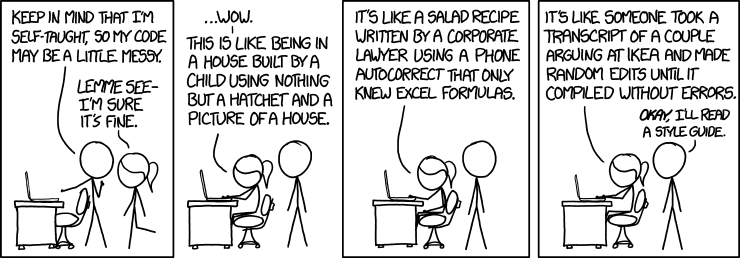
\includegraphics[width=\linewidth]{./gfx/xkcd-codeQuality}
\caption
	[Code Quality]
	{Code Quality. Quelle: \url{https://xkcd.com/1513/}}
\end{center}
\end{figure}
Immer wieder wird die Frage gestellt, welche Programmteile sinnvoll in Funktionen ausgelagert werden sollten. Während es dafür keine allgemeingültige Formel gibt, kann man zumindest einige Situationen aufzählen, in denen es sich anbietet, Code in einer eigenen Funktion anzulegen.

Generell ist es sinnvoll, alle Arbeitsschritte, die eine gedankliche Einheit bilden, in einer Funktion zu verkapseln. Eine gedankliche Einheit ist etwa \enquote{Berechne den Wert einer Funktion} oder \enquote{Gib Text auf dem Bildschirm aus}.

Insbesondere sollte aller Code, den man mehrfach verwenden will in Funktionen stehen. Kopierter Code macht das Programm länger und damit schwieriger zu warten. Vor allem aber ergibt sich daraus eine Fehlerquelle, da Änderungen an einem kopierten Codeteil verlangen, auch alle anderen Stellen zu ändern, an denen diese Kopien auftauchen. Es ist leicht, diese Stellen zu vergessen und so inkonsistenten und fehlerhaften Code zu erhalten.

Schließlich kann es von Vorteil sein, selbst Codeblöcke in Funktionen zu setzen, die nur einmal aufgerufen werden. Ein Funktionsname sollte eindeutig beschreiben, welche Aufgabe die Funktion erfüllt. Ist dies gegeben, so kann der Ablauf eines Programms klarer im Code gelesen werden, ohne im Detail Zeile für Zeile nachvollziehen zu müssen. Sehen Sie sich dazu folgenden Code an:

\begin{codebox}[Beispiel: \texttt{main} eines Spiels]
\begin{minted}[linenos]{c}
/* ... #include-Zeilen stehen hier ... */

/* ... Funktionen stehen hier ... */

int main () {
  showTitleAnimation();
  
  do {
    int selectedMenuPoint = 0;
    
    showMenuScreen();
    selectedMenuPoint = askForMenuOption();
    
    performAction(selectedMenuPoint);
  } while(selectedMenuPoint);
}
\end{minted}
\end{codebox}

Hier wird vor Start des Spiels eine Animation gezeigt. Im Anschluss wird jeweils in Folge ein Menübildschirm dargestellt, eine Usereingabe angenommen und dann dafür gesorgt, dass die Auswahl des Users ausgeführt wird. Dies wird solange durchgeführt, bis die Funktion \texttt{askForMenuOption} den Wert \texttt{0} zurückgibt. Dies könnte (und sollte) \eg dann der Fall sein, wenn der User auswählt, das Spiel zu beenden.

Obwohl in diesem Beispiel nicht klar ist, wie die Animation im Detail aussieht, oder welche Menüpunkte angeboten werden, ist klar, wie das Programm organisiert ist. Neue Features können leicht eingefügt werden. Soll etwa eine Animation ausgeführt werden, sobald ein Menupunkt ausgewählt wurde, so kann nach Zeile 12 noch eine neue Funktion \texttt{showMenuAnimation(selectedMenuPoint)} eingefügt werden.

Funktionen können sich auch untereinander aufrufen, wie wir im Abschnitt \ref{sec:forwardDeclaration} gesehen haben. Dies \enquote{kostet} einigen Verwaltungsaufwand (um den wir als ProgrammiererInnen uns aber nicht explizit kümmern müssen). Der Compiler muss für jeden Aufruf einer Funktion mitspeichern, an welche Stelle bei Verlassen der aufgerufenen Funktion zurück gesprungen werden soll; außerdem müssen die Speicherbereiche für die einzelnen Funktionen angelegt und wieder frei gegeben werden. Bei geringer \emph{Aufruftiefe} (bis etwa 20 Aufruf-Ebenen) fällt dies nicht weiter ins Gewicht. Stärkere Verschachtelung macht Programme aber merklich langsamer. Natürlich ist es vor allem schwierig, eine Struktur mit so vielen Ebenen zu überblicken. Daher möchte ich Ihnen diesen Gedanken als einzige Beschränkung für die Sinnhaftigkeit von Funktionen mitgeben: halten Sie die Verschachtelung klein und übersichtlich. In Kapitel \ref{chp:recursion} werden wir diesen Gedanken nochmals aufgreifen.

\subsection{Rückgabe mehrerer Werte}
Eine Funktion kann nur entweder nichts (\mintinline{c}{void}) oder genau einen einzigen Wert zurückgeben. Es gibt aber Situationen, in denen dieselbe Funktion \emph{mehrere} Werte zugleich berechnen soll. Um dies zu ermöglichen stehen uns zwei Techniken zur Verfügung: Wir können ein \emph{Array} oder ein \mintinline{c}{struct} zurückgeben.

Arrays werden über Pointer verwaltet, daher muss der Rückgabetyp auch ein Pointer sein. (Tatsächlich gibt unsere Funktion also nur einen einzigen Wert zurück; dieser gibt dann aber eine Speicherstelle an, an der alle berechneten Werte zu finden sind.)

Sehen Sie sich folgendes Beispiel an, das ein Rezept für Obstsalat auf verschiedene Menschenmengen anpasst:

\begin{codebox}[Beispiel: Umrechnung eines Rezepts]
\begin{minted}[linenos]{c}
#include <stdio.h>
#include <stdlib.h>
// https://www.chefkoch.de/rezepte/654221166964999/Bunter-Obstsalat.html

double * fruitsaladForPersons(double persons) {
  double * reVal = malloc(8 * sizeof(*reVal));
  
  reVal[0] = persons/4.0 *   3;  // apples
  reVal[1] = persons/4.0 *   2;  // bananas
  reVal[2] = persons/4.0 *   2;  // peaches
  reVal[3] = persons/4.0 *   2;  // kiwis
  reVal[4] = persons/4.0 *   1;  // mangos
  reVal[5] = persons/4.0 *   1;  // oranges
  reVal[6] = persons/4.0 * 200;  // grams of grapes
  reVal[7] = persons/4.0 *  50;  // grams of walnuts
  
  return reVal;
}

int main () {
  double persons = 2;
  double * requirements = fruitsaladForPersons(persons);
  
  printf("Obstsalat für %1.0lf Personen:\n", persons);
  printf("\tÄpfel    : %5.1lf\n"  , requirements[0]);
  printf("\tBananen  : %5.1lf\n"  , requirements[1]);
  printf("\tPfirsiche: %5.1lf\n"  , requirements[2]);
  printf("\tKiwis    : %5.1lf\n"  , requirements[3]);
  printf("\tMangos   : %5.1lf\n"  , requirements[4]);
  printf("\tOrangen  : %5.1lf\n"  , requirements[5]);
  printf("\tTrauben  : %5.1lf g\n", requirements[6]);
  printf("\tWalnüsse : %5.1lf g\n", requirements[7]);
  
  free(requirements);
}
\end{minted}
\end{codebox}

\begin{cmdbox}[Ausführungsbeispiel: Umrechnung eines Rezepts]
\begin{minted}{text}
Obstsalat für 2 Personen:
        Äpfel    :   1.5
        Bananen  :   1.0
        Pfirsiche:   1.0
        Kiwis    :   1.0
        Mangos   :   0.5
        Orangen  :   0.5
        Trauben  : 100.0 g
        Walnüsse :  25.0 g
\end{minted}
\end{cmdbox}

Beachten Sie hier auch, dass der in Zeile 5 reservierte Speicherbereich wieder freigegeben werden muss. Dies geschieht in Zeile 35.

\mintinline{c}{struct}s werden in Kapitel \ref{chp:structs} besprochen.

\subsection{Speicherklasse \mintinline{c}{static}} \label{sec:staticVar}
Variablen sind immer nur in ihrem aktuellen Scope sichtbar, und werden \idR zerstört, sobald der aktuelle Scope verlassen wird. Manchmal soll aber der Wert einer Speicherstelle erhalten bleiben, selbst wenn die Ausführung den Scope verlässt, in dem die Variable definiert wurde. Bisher können wir dies nur lösen, indem wir die entsprechende Variable in einem Scope anlegen, das für die gesamte Lebensdauer des Programms existiert (also in der \texttt{main} oder als globale Variable), und einen Pointer auf diesen Wert \enquote{durchreichen}.

\begin{codebox}[Beispiel: Funktionsaufrufe mitzählen (1)]
\begin{minted}[linenos]{c}
#include <stdio.h>

void foobar(int * callCounter) {
  (*callCounter)++;
  printf("Aufruf #%d\n", *callCounter);
}

int main () {
  int calls = 0;
  
  foobar(&calls);
  foobar(&calls);
}
\end{minted}
\end{codebox}

\begin{cmdbox}[Ausführungsbeispiel: Funktionsaufrufe mitzählen (1)]
\begin{minted}{text}
Aufruf #1
Aufruf #2
\end{minted}
\end{cmdbox}

Dieser Code funktioniert zwar, ist aber fehleranfällig. Zunächst muss ein Anwender den Zweck von \texttt{calls} kennen, um die Funktion \texttt{foobar} richtig zu nutzen. Insbesondere darf \texttt{calls} nicht versehentlich geändert werden. Nicht zuletzt \enquote{belegt} diese Technik einen Variablennamen in der \texttt{main}.

Als Alternative dazu können Variablen in der Funkton \texttt{foobar} mit dem Schlüsselwort \mintinline{c}{static} deklariert werden. Auf diese Weise bleibt die Speicherstelle reserviert, \ie gespeicherte Werte erhalten, auch wenn die Funktion später wieder aufgerufen wird. Der Scope-Mechanismus hingegen wird nicht außer Kraft gesetzt. In Code sieht das dann so aus:

\begin{codebox}[Beispiel: Funktionsaufrufe mitzählen (2)]
\begin{minted}[linenos]{c}
#include <stdio.h>

void foobar() {
  static int callCounter = 0;
  callCounter++;
  printf("Aufruf #%d\n", callCounter);
}

int main () {
  foobar();
  foobar();
  // printf("%d\n", callCounter); -- unzulässig, falscher Scope
}
\end{minted}
\end{codebox}

Der Compiler legt \emph{ein einziges Mal} die Speicherstelle für \texttt{callCounter} an, selbst, wenn (wie hier) die Funktion \texttt{foobar} mehrfach aufgerufen wird. Entsprechend findet auch die Wertzuweisung in Zeile 4 nur ein einziges Mal statt. Danach \enquote{erinnert} sich der Compiler an die bereits angelegte Speicherstelle, sobald \texttt{foobar} \enquote{betreten} wird, und \enquote{vergisst} diesen Variablennamen (nicht aber die Speicherstelle selbst) wieder, wenn die Funktion verlassen wird.

\section{Optimierung: \mintinline{c}{inline}} \label{sec:inline}
Bei einem Funktionsaufruf werden die Werte von Parametern kopiert und die Stelle gespeichert, von der weg gesprungen wurde, so dass beim Verlassen der Funktion die Ausführung nach dem Sprung-Befehl fortgesetzt werden kann. Dieses Kopieren und Speichern kostet Zeit. Bei häufig wiederkehrenden Aufrufen führt dies zu merklichen Performance-Einbrüchen.

Um dem entgegen zu wirken, können \emph{kurze} Funktionen als \mintinline{c}{inline} deklariert werden. Dies teilt dem Compiler mit, dass der Funktionskörper an der aufrufenden Stelle eingefügt werden sollte, statt einen normalen Sprung und Rücksprung durchzuführen. Ergebnis ist eine größere ausführbare Datei (da derselbe Code an mehreren Stellen eingefügt wird), der aber schneller läuft. Für die ProgrammiererInnen ergibt sich sonst kein Unterschied -- Funktionsaufruf sowie Scoping funktionieren wie bisher besprochen.

Um eine Funktion als \mintinline{c}{inline} zu deklarieren, schreibt man eine forward declaration und stellt dieser das Schlüsselwort \mintinline{c}{inline} voran:

\begin{codebox}[Syntax: \texttt{inline}-Funktion]
\begin{minted}{c}
inline Rückgabetyp Funktionsname (Parameterliste);
\end{minted}
\end{codebox}

\begin{codebox}[Beispiel: Maximum von zwei Ganzzahlen finden]
\begin{minted}[linenos]{c}
inline int max (int a, int b);
       int max (int a, int b) {return a > b   ?   a  :  b;}
\end{minted}
\end{codebox}

\section{Funktionszeiger} \label{sec:funcPtr}
Alle \enquote{Dinge}, mit denen wir arbeiten, müssen im Speicher abgelegt werden, und haben daher notwendigerweise auch eine Adresse. Dies umfasst einzelne Zahlen, Gruppen von Zahlen (Arrays) und eben auch Programmcode. Bei der Ausführung eines Programms wird dieses zunächst in den Arbeitsspeicher kopiert, und dann die Maschinencode-Anweisungen ausgeführt, die in der Datei vermerkt waren. Wir können daher auch die Adressen von bestimmten Programmteilen ausfindig machen und mit der Ausführung an diese Adressen springen. Zu diesem Zweck existiert das Konzept von \texttt{Funktionszeigern}, also Pointer auf Funktionen.

Funktionszeiger sind wie alle Pointer Variablen, die zunächst deklariert werden müssen. Diese Deklaration enthält alle Informationen der Funktionssignatur, also Rückgabewert der Funktion und Parameterliste. Dies drückt sich in der folgenden (leider etwas unhandlichen Syntax) aus:
\begin{codebox}[Syntax: Deklaration Funktionszeiger]
\begin{minted}{c}
Rückgabetyp (*Variablenname) (Parameterliste);
\end{minted}
\end{codebox}

Solchen Variablen kann nun die Adresse einer beliebigen Funktion (mit passender Signatur) zugewiesen werden. Dies geschieht \emph{ohne} jegliche Operatoren, einfach über den Funktionsnamen:

\begin{codebox}[Beispiel: Funktionszeiger (1)]
\begin{minted}[linenos]{c}
#include <stdio.h>

void foo() {
  printf("blerb.\n");
}

int main () {
  void (*funcPtr)() = foo;
}
\end{minted}
\end{codebox}

Der Codeabschnitt, auf den dieser Funktionspointer zeigt, kann nun mit dem neuen Symbol \texttt{funcPtr} aufgerufen werden, ganz als würde man direkt mit \texttt{foo} arbeiten:

\begin{codebox}[Beispiel: Funktionszeiger (2)]
\begin{minted}[linenos]{c}
#include <stdio.h>

void foo() {
  printf("blerb.\n");
}

int main () {
  void (*funcPtr)() = foo;
\end{minted}
\end{codebox}
%
\begin{codebox}[]
\begin{minted}[linenos]{c}
  printf("direkt : ");
  foo();
  
  printf("funcPtr: ");
  funcPtr();
}
\end{minted}
\end{codebox}

\begin{cmdbox}[Ausführungsbeispiel: Funktionszeiger (2)]
\begin{minted}{text}
direkt : blerb.
funcPtr: blerb.
\end{minted}
\end{cmdbox}

\begin{hintbox}
Der Name einer Funktion beschreibt selbst einen Funktionszeiger! Der Aufruf einer Funktion ist eine \emph{Operation}, vergleichbar mit dem Dereferenzieren (Operator \texttt{*}). Daher müssen auch Funktionen, die keine Parameter erwarten, mit leeren Klammern () aufgerufen werden.
\end{hintbox}

Der Zweck dieser Technik ist, das Verhalten anderer Funktionen vom Ergebnis anderer Berechnungen abhängig zu machen, ohne sich dabei auf die Art der Berechnung festzulegen.

Als Beispiel sei die Funktion \texttt{qsort}\footnote{Der Sortieralgorithmus \emph{quicksort}, der dieser Funktion zugrunde liegt, wird in der Vorlesung \emph{Algorithmen und Datenstrukturen} an der Universität Regensburg genauer besprochen.} genannt (definiert in \texttt{stdlib.h}). Diese Funktion kann Arrays beliebigen Typs nach beliebigen Kriterien sortieren. Die Sortier-Kriterien werden in Form einer Funktion \texttt{comp} beschrieben, die zwei Werte \texttt{a} und \texttt{b} miteinander vergleicht. (Hier verwende ich den Namen \texttt{comp}, um den folgenden Abschnitt leichter lesbar zu halten; die Vergleichsfunktion darf in der Anwendung aber einen beliebigen Namen haben.)

Da Arrays \emph{beliebigen} Typs sortiert werden, können an \texttt{comp} nicht die \emph{Werte} \texttt{a} und \texttt{b} übergeben werden, sondern nur ihre \emph{Adressen} \texttt{\&a} und \texttt{\&b}.

Wenn \texttt{a} \emph{vor} \texttt{b} in der sortierten Liste auftauchen soll, soll der Rückgabewert von \texttt{comp(\&a, \&b)} gleich \texttt{-1} sein. Falls dagegen \texttt{b} vor \texttt{a} sortiert werden soll, so muss \texttt{+1} zurückgegeben werden. Schließlich wird \texttt{comp} den Wert \texttt{0} zurückgeben, wenn \texttt{a} und \texttt{b} gleichwertig sind. (\emph{Gleichwertig} bedeutet in diesem Kontext nicht zwingend \emph{gleich}. Wir könnten zum Beispiel Zahlen nach ihrer Quersumme sortieren. Für diese Sortierung sind die Zahlen \texttt{19} und \texttt{91} dann gleichwertig, nicht aber gleich.) 

Die \href{https://en.cppreference.com/w/c/algorithm/qsort}{cpp-Referenz} teilt uns die Signatur der Funktion \texttt{qsort} mit:

\begin{codebox}[Prototyp der Funktion \texttt{qsort}]
\begin{minted}{c}
void qsort( void * ptr, size_t count, size_t size,
            int (*comp)(const void *, const void *) );
\end{minted}
\end{codebox}

Betrachten wir die einzelnen Parameter:
\begin{itemize}
\item Der erste Parameter \texttt{ptr} ist ein Pointer auf ein beliebiges Array und daher vom Typ
		\mintinline{c}{void *}. 
\item Mit \texttt{count} wird die Zahl der Elemente des Arrays beschrieben. (Der Typ 
		\mintinline{c}{size_t} ist ein Alias (ein alternativer Name) für \mintinline{c}{unsigned int}.)
\item Der Wert \texttt{size} beschreibt den Speicherbedarf \emph{eines} Elements des Arrays. Wir
		brauchen diese Information, da \texttt{qsort} \ua für \mintinline{c}{int}-, 
		\mintinline{c}{double}- oder \mintinline{c}{char}-Arrays funktionieren soll, die allesamt 
		unterschiedlichen Speicherbedarf haben.
\item Die letzte Zeile schließlich benennt den Parameter \texttt{comp}, der eine Vergleichsfunktion
		benennt. Diese Funktion wird einen \mintinline{c}{int} zurück geben, und nimmt zwei
		\mintinline{c}{const void *} als Argumente an. Dabei bedeutet \mintinline{c}{const} wieder, dass
		\texttt{comp} die Werte von \texttt{a} und \texttt{b} nur lesen, nicht aber verändern wird.
		Der Modifier \mintinline{c}{const} gehört zum Datentyp und muss daher auch in unserer Funktions-
		Signatur auftauchen. Wieder gilt: Da der Datentyp von \texttt{a} und \texttt{b} beliebig ist,
		können nur \mintinline{c}{void *} übergeben werden.
\end{itemize}

Mit diesen Informationen können wir das (leicht abgewandelte) Beispiel von der \href{https://en.cppreference.com/w/c/algorithm/qsort}{cpp-Referenz} verstehen:

\begin{codebox}[Beispiel: \texttt{qsort} mit zwei Sortiermethoden]
\begin{minted}[linenos]{c}
#include <stdio.h>
#include <stdlib.h>
 
int comp_ascending(const void* a, const void* b) {
    int arg1 = *(const int *) a;
    int arg2 = *(const int *) b;
 
    if (arg1 < arg2) return -1;
    if (arg1 > arg2) return  1;
    return 0;
}

int comp_descending(const void* a, const void* b) {
    return -comp_ascending(a, b);
}

int main(void) {
    int ints[] = { -2, 99, 0, -743, 2, 4 };
    int size = sizeof(ints) / sizeof(*ints);
    
    printf("Aufsteigende Sortierung:\n");
    qsort(ints, size, sizeof(int), comp_ascending);
    
    for (int i = 0; i < size; i++) {
        printf("%d ", ints[i]);
    }
    printf("\n");
    
    printf("Absteigende Sortierung:\n");
    qsort(ints, size, sizeof(int), comp_descending);
    
    for (int i = 0; i < size; i++) {
        printf("%d ", ints[i]);
    }
    printf("\n");
}
\end{minted}
\end{codebox}

\begin{cmdbox}[Ausführungsbeispiel: \texttt{qsort} mit zwei Sortiermethoden]
\begin{minted}{text}
Aufsteigende Sortierung:
-743 -2 0 2 4 99 
Absteigende Sortierung:
99 4 2 0 -2 -743 
\end{minted}
\end{cmdbox}

Obwohl die Funktion \texttt{qsort} nur einmal programmiert wurde, kann sie mit diesen Techniken also \emph{generisch} benutzt werden, \ie sie ist für viele verschiedene Zwecke einsetzbar, die bei der Erstellung von \texttt{qsort} noch nicht einmal vorgesehen waren.